\section{Battery Models and Robustness}
\subsection{Kinetic Battery Model}

\begin{frame}[fragile]{Battery Models}{\insertsubsection}
	\centering
	\begin{equation*}
	y_1(t) = c*C*e^{-k't}+\frac{(C*k'c-I)(1-e^{-k't})}{k'}-\frac{I*c(k't-1+e^{-k't})}{k'}
	\end{equation*}\quad
	\begin{equation*}
	y_2(t) = (1-c)C*e^{-k't}+C(1-c)(1-e^{-k't})-\frac{I(1-c)(k't-1+e^{-k't})}{k'}
	\end{equation*}\quad
	\begin{equation*}
	a '== -i+k*(b/(1-c)-a/c)
	\end{equation*}\quad
	\begin{equation*}
	b '== -k*(b/(1-c)-a/c)+(insolation*RechargeRate)
	\end{equation*}
\end{frame}

\begin{frame}[fragile]{Battery Models}{\insertsubsection}
	\centering
	\begin{figure}[h]
		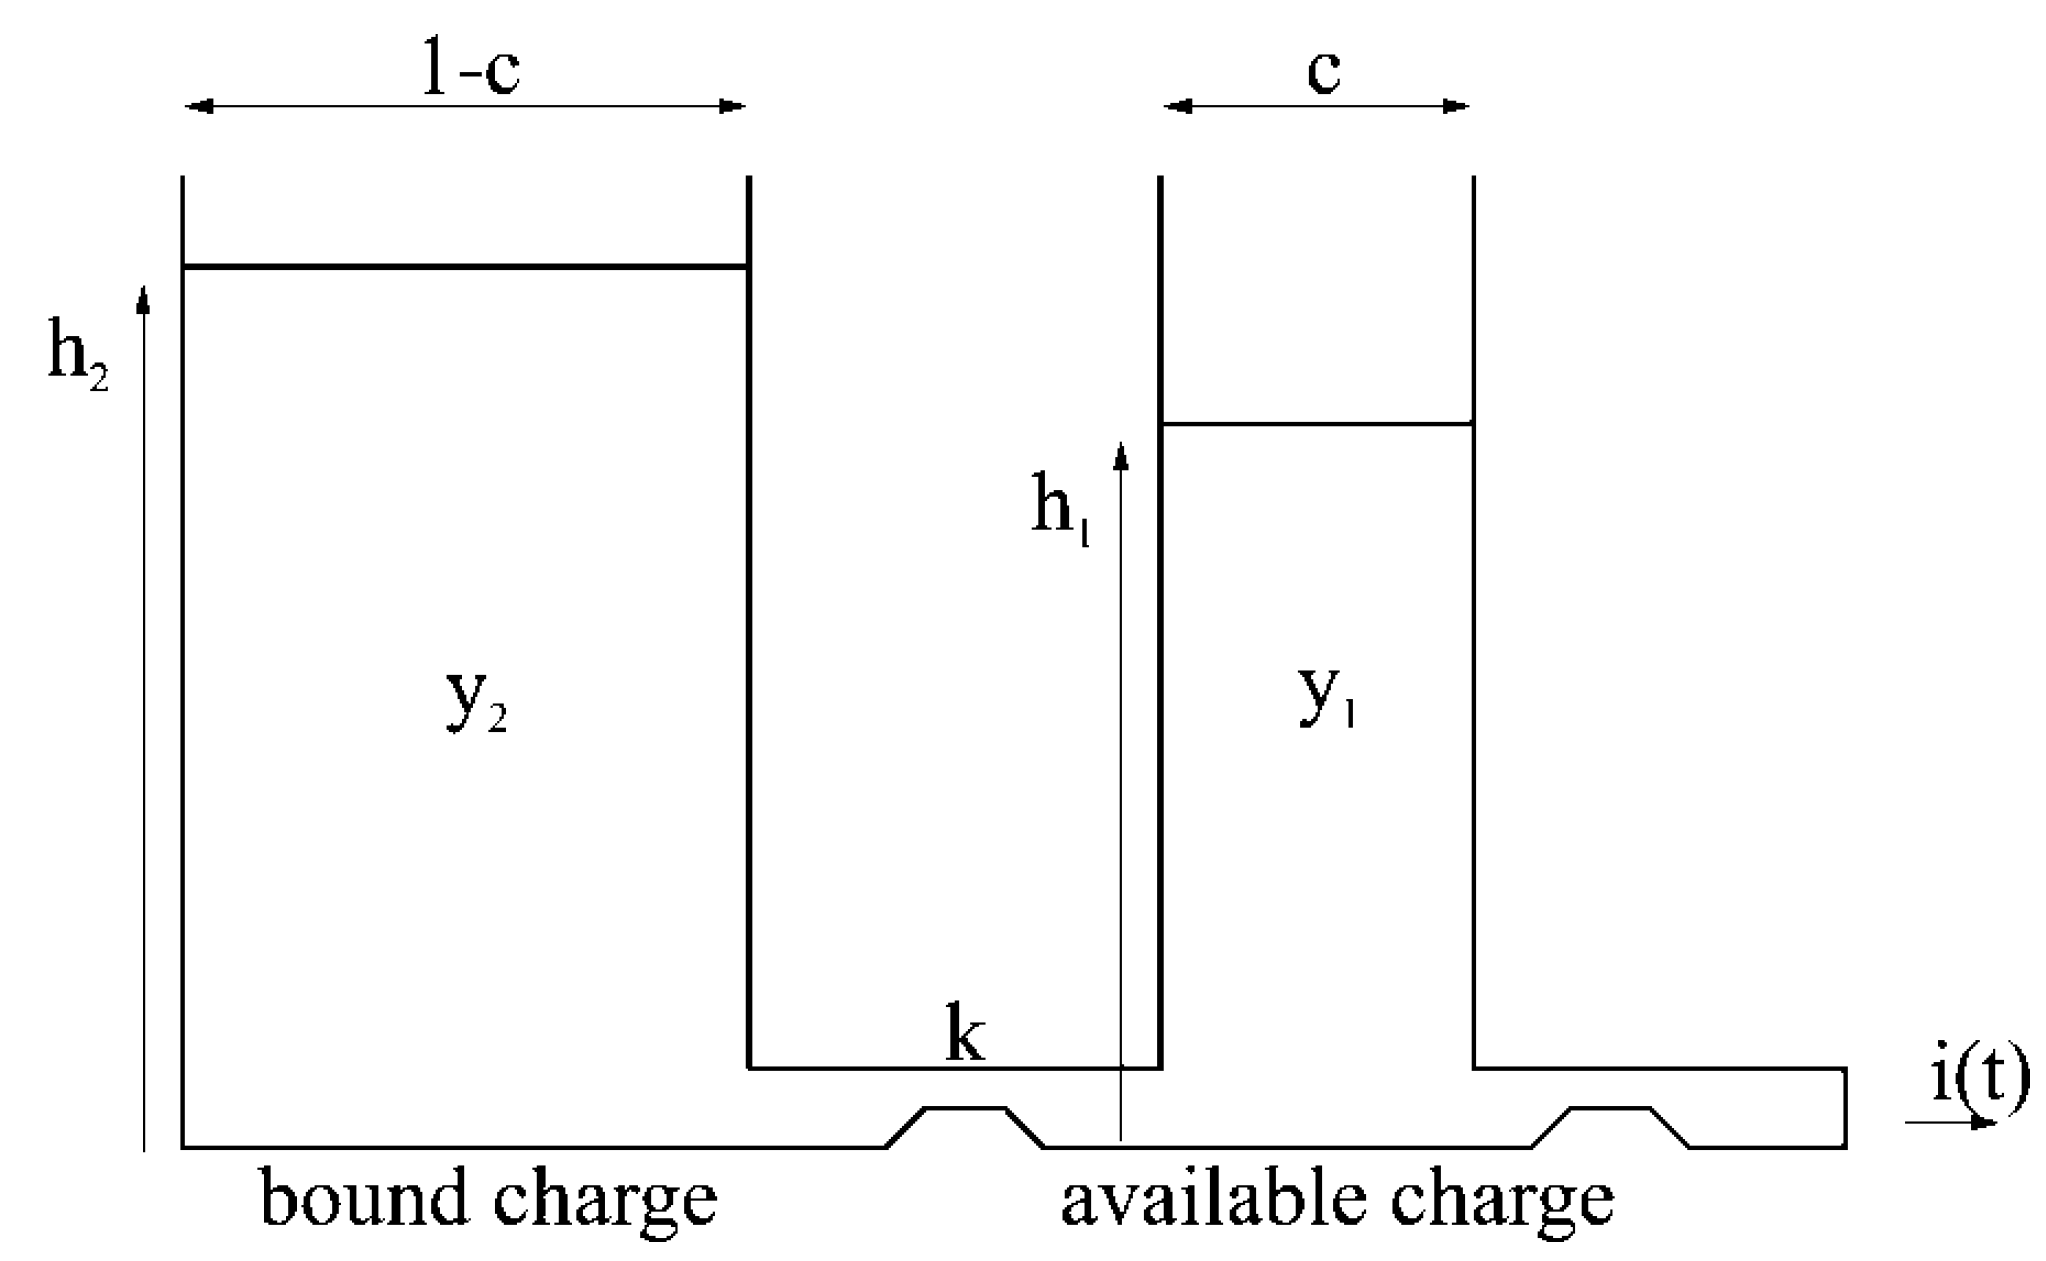
\includegraphics[width=.7\textwidth]{graphics/kibam_wells}
	\end{figure}
	\begin{equation*}
	y_1(t) = c*C*e^{-k't}+\frac{(C*k'c-I)(1-e^{-k't})}{k'}-\frac{I*c(k't-1+e^{-k't})}{k'}
	\end{equation*}
	\begin{equation*}
	y_2(t) = (1-c)C*e^{-k't}+C(1-c)(1-e^{-k't})-\frac{I(1-c)(k't-1+e^{-k't})}{k'}
	\end{equation*}
\end{frame}
\note{e growth, rate of change (compound interest)}
\begin{frame}[fragile]{Battery Models}{\insertsubsection}
	\centering
	\begin{figure}[h]
		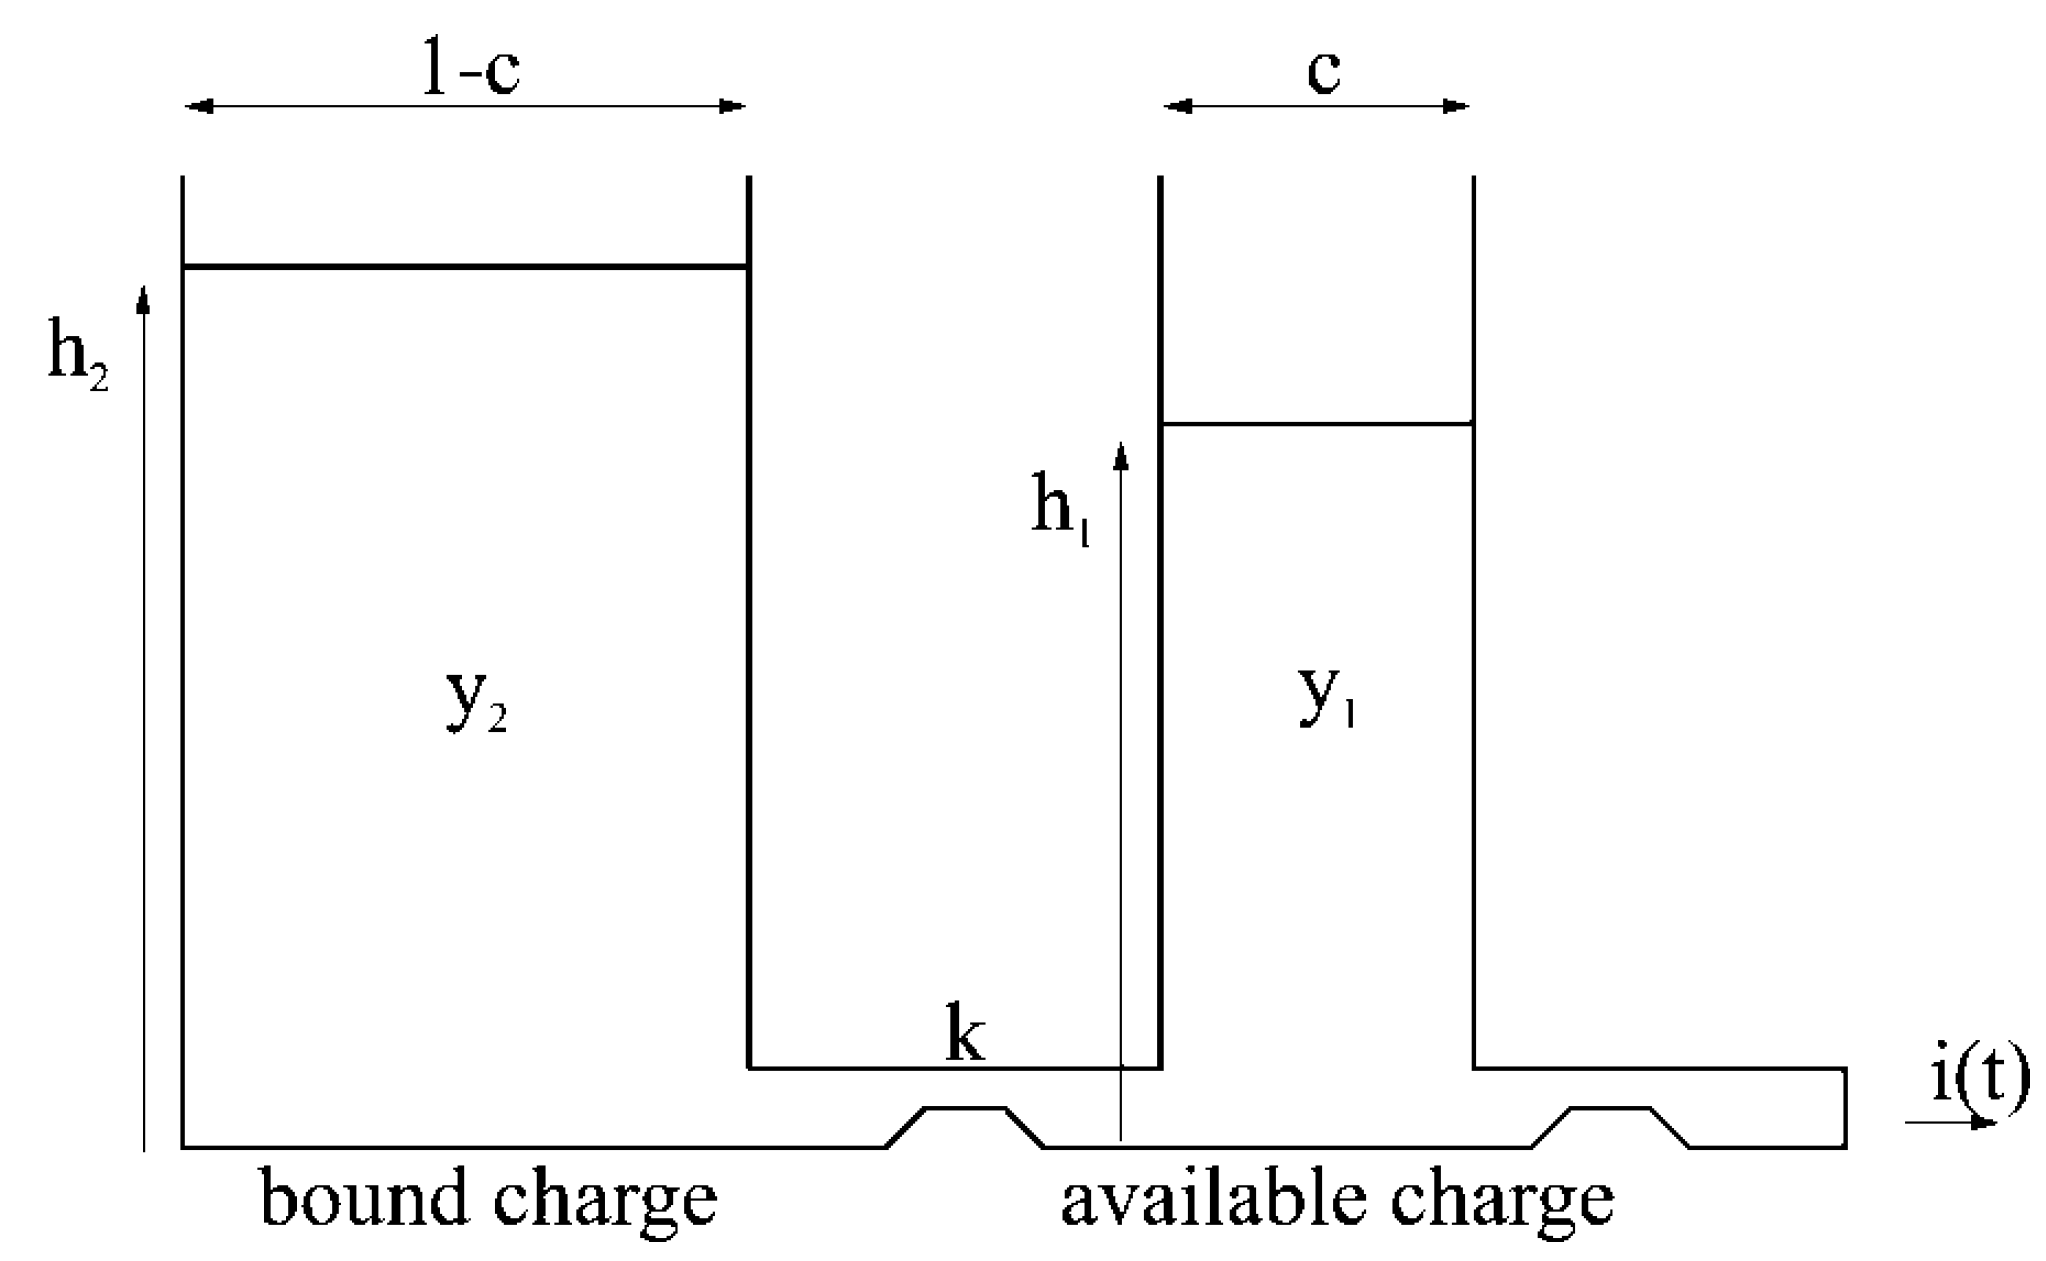
\includegraphics[width=.7\textwidth]{graphics/kibam_wells}
	\end{figure}
	\begin{equation*}
\frac{dy_1}{dt} = -i(t)+k(h_2-h_1)
	\end{equation*}
	\begin{equation*}
\frac{dy_2}{dt} = -k(h_2-h_1)
	\end{equation*}
\end{frame}

\begin{frame}[fragile]{Battery Models}{\insertsubsection}
	Calculate height of $h_1$ and $h_2$
	\begin{equation*}
	h_1 = y_1/c
	\end{equation*}
	\begin{equation*}
	h_2 = y_2/1-c
	\end{equation*}\quad
	\begin{equation*}
	 \frac{dy_1}{dt} = -i(t)+k(h_2-h_1)
	\end{equation*}	
	\begin{equation*}
	\xrightarrow[dt]{} dy_1 = -i+k(h_2-h_1) 
	\end{equation*}
	\begin{equation*}
	\xrightarrow[h_1, h_2]{} dy_1 = -i+k(y_2/(1-c)-y_1/c)
	\end{equation*}
	\begin{equation*}
	\xrightarrow[y_1, y_2]{} da = -i+k(b/(1-c)-a/c)
	\end{equation*}
	\begin{equation*}
	a '== -i+k(b/(1-c)-a/c)
	\end{equation*}
\end{frame}

\begin{frame}[fragile]{Battery Models}{\insertsubsection}
	\begin{equation*}
	db = -k(b/1-c-a/c)
	\end{equation*}
	\begin{equation*}
	b '== -k*(b/(1-c)-a/c)+(insolation*RechargeRate)
	\end{equation*}
	\begin{figure}[h]
		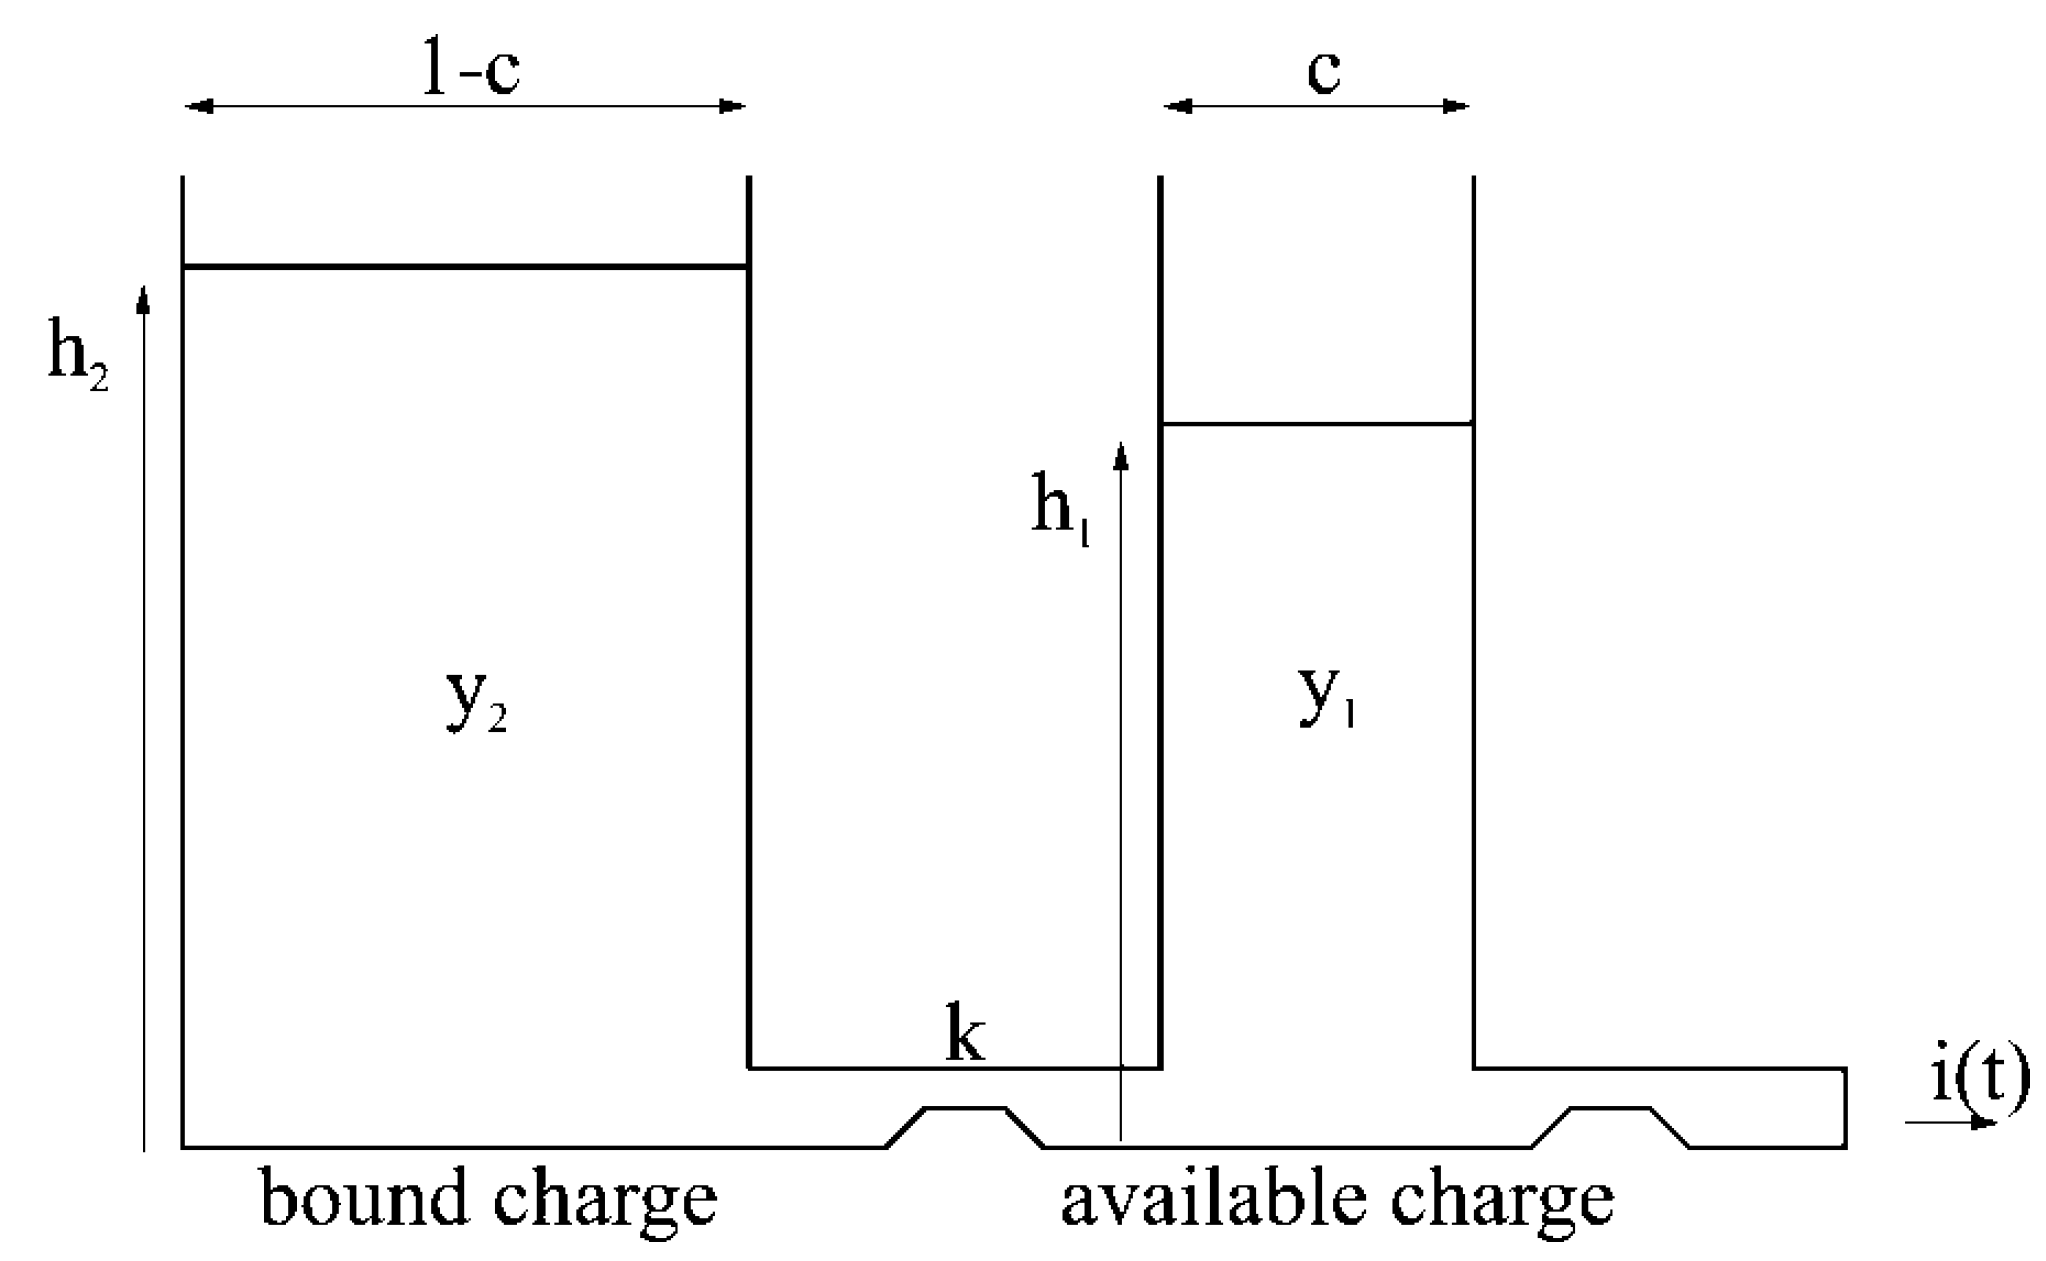
\includegraphics[width=.7\textwidth]{graphics/kibam_wells}
	\end{figure}
\end{frame}
\note{Talk about the inaccuarcy, we recharged energy is added to bound charge}

\subsection{Chose of Battery Model}
\begin{frame}[fragile]{Battery Models}{\insertsubsection}
\begin{table}[]
	\centering
	\begin{tabular}{lllll}
		\multicolumn{5}{c}{Variable load} \\
		\rowcolor[HTML]{EFEFEF} 
		Test & Meas, min & \%$\Delta$ Ideal & \%$\Delta$ Peukert & \%$\Delta$ KiBaM \\
		C1 & 54.5 & 29.91\% & 11.01\% & -33.39\% \\
		\rowcolor[HTML]{EFEFEF} 
		C2 & 73.3 & 25.38\% & 7.91\% & -24.01\% \\
		C3 & 88.3 & 22.88\% & 6.23\% & -19.14\% \\
		\rowcolor[HTML]{EFEFEF} 
		C4 & 136.0 & 19.85\% & 4.78\% & -9.12\% \\
		C5 & 182.7 & 18.50\% & 4.11\% & -3.83\% \\
		\rowcolor[HTML]{EFEFEF} 
		C6 & 59.0 & 26.61\% & 9.15\% & -30.34\% \\
		C7 & 51.1 & 30.92\% & 10.57\% & -40.31\% \\
		\rowcolor[HTML]{EFEFEF} 
		C8 & 55.0 & 28.73\% & 10.00\% & -30.73\% \\
		C9 & 54.9 & 28.96\% & 10.20\% & -36.61\% \\
		\rowcolor[HTML]{EFEFEF} 
		C10 & 142.7 & 20.04\% & 4.27\% & -7.71\%
	\end{tabular}
\end{table}
\end{frame}

\subsection{Functions and Variables}
\begin{frame}[fragile]{Robustness}{\insertsubsection}
	\centering
	\begin{figure}[h]
		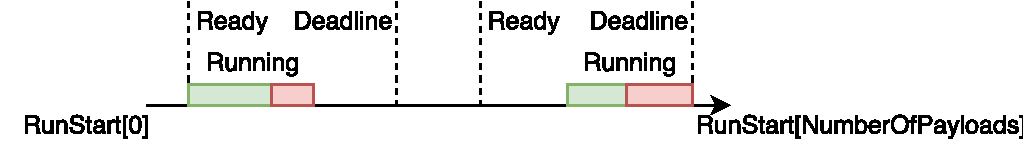
\includegraphics[width=1\textwidth]{graphics/payload_execution}
	\end{figure}
	\begin{figure}[h]
		\begin{minipage}{.7\textwidth}
		\begin{lstlisting}
N = 2;
Payloads[N][3] = {{10,15,20}, {7,15,20};
RunStart[NumberOfPayloads] = {50,100};
		\end{lstlisting}
		\end{minipage}\\
		\begin{minipage}{.7\textwidth}
			\begin{lstlisting}
void enqueue(){
	i = IIdle + Costs[active];
	B = Payloads[active][0];
	W = Payloads[active][1];
}
			\end{lstlisting}
		\end{minipage}
	\end{figure}
\end{frame}

\subsection{Processor}
\begin{frame}[fragile]{Robustness}{\insertsubsection}
\begin{figure}[H]
	\centering
	\begin{figure}[h]
		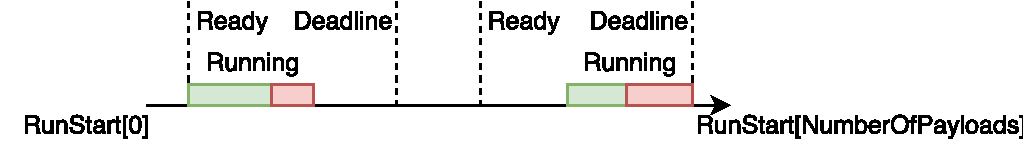
\includegraphics[width=.8\textwidth]{graphics/payload_execution}
	\end{figure}\quad
	\scalebox{.6}{
	\begin{tikzpicture}
	%Locations
	\node [init] (l0) [label={[align=left]above:\textcolor{name}{Init}}] {$\cup$};
	\node [location] (l1) [right of=l0, xshift=40mm, label={
		[align=left]above:
		\textcolor{name}{Idle}},
	label={
		[align=center]below:
		\textcolor{invariant}{totalTime <= RunStart[payloadNumber]}
	}] {};
	\node [location] (l2) [right of=l1, xshift=80mm, label={
		[align=left]above:
		\textcolor{name}{Ready}
	}] {};
	\node [location] (l3) [below of=l0, yshift=-40mm, label={
		[align=left]below:
		\textcolor{name}{Done}
	}] {};
	\node [location] (l4) [below of=l1, yshift=-40mm, label={
		[align=left]below:
		\textcolor{name}{Wait}\\
		\textcolor{invariant}{x <= D}
	}] {};
	\node [location] (l5) [below of=l2, yshift=-40mm, label={
		[align=left]below:
		\textcolor{name}{Running}\\
		\textcolor{invariant}{x <= W}
	}] {};
	\path[->,black, thick] (l0) edge node [midway, above][align=left]{
		\textcolor{update}{t=0,i = IIdle,}\\
		\textcolor{update}{setActive()}} (l1);
	\path[->,black, thick] (l1) edge node [midway, above][align=center]{
		\textcolor{guard}{totalTime >=RunStart[payloadNumber]}\\
		\textcolor{sync}{ready!}\\
		\textcolor{update}{x=0, t=0,}\\
		\textcolor{update}{deadline()}} (l2);
	\path[->,black, thick] (l2) edge node [midway, right][align=left]{
		\textcolor{sync}{run?}\\
		\textcolor{update}{x := 0,}\\
		\textcolor{update}{setActive(),}\\
		\textcolor{update}{enqueue()}\\
		\textcolor{update}{earnings +=}\\
		\textcolor{update}{Profit[active]}} (l5);
	\path[->,black, thick] (l2) edge node [midway, left][align=left]{
		\textcolor{sync}{skip?}\\
		\textcolor{update}{payloadNumber ++,}\\
		\textcolor{update}{skipped()}} (l4);
	\path[->,black, thick] (l5) edge node [midway, below][align=left]{
		\textcolor{guard}{x >= B}\\
		\textcolor{update}{dequeue(), active = -1,}\\
		\textcolor{update}{payloadNumber ++}} (l4);
	\path[->,black, thick] (l4) edge node [midway, left][align=left]{
		\textcolor{guard}{x >= D \&\&}\\
		\textcolor{guard}{!done()}\\
		\textcolor{update}{setActive()}} (l1);
	\path[->,black, thick] (l4) edge node [midway, below][align=left]{
		\textcolor{guard}{done()}\\
		\textcolor{update}{on = false,}\\
		\textcolor{update}{active = -1}} (l3);
	\end{tikzpicture}}
\end{figure}
\end{frame}

\subsection{Queries}
\begin{frame}[fragile]{Robustness}{\insertsubsection}
	\centering
	
\end{frame}

